\chapter{Authentication methods}

The \tls{} protocol provides confidentiality and encryption, but
also offers authentication, which is a prerequisite
for a secure connection. 
The available authentication methods in \gnutls{} are:
\begin{enumerate}
 \item Certificate authentication
 \item Anonymous authentication
 \item SRP authentication
\end{enumerate}

% x.509 section
\section{Authentication using X.509\index{X.509 certificates} certificates}

This authentication method is part of the certificate authentication
method in \gnutls{}.
\par
X.509 certificates contain the public parameters, 
of a public key algorithm, and the authority's signature, which proves the
authenticity of the parameters.
\par
The key exchange methods shown in \hyperref{figure}{figure }{}{fig:cert} are
available in X.509 authentication. 

See \ref{x509:trust} on page \pageref{x509:trust} for more information
on X.509 protocols.


\begin{figure}[hbtp]
\index{Key exchange algorithms}
\begin{tabular}{|l|p{9cm}|}
\hline
RSA & The RSA algorithm is used to encrypt a key and send it to the peer.
The certificate must allow the key to be used for encryption.
\\
\hline
RSA\_EXPORT & The RSA algorithm is used to encrypt a key and send it to the peer.
In the EXPORT algorithm, the server signs temporary RSA parameters of 512
bits -- which are considered weak -- and sends them to the client.
\\
\hline
DHE\_RSA & The RSA algorithm is used to sign Ephemeral Diffie Hellman
parameters which are sent to the peer. The key in the certificate must allow
the key to be used for signing. Note that key exchange algorithms which use
Ephemeral Diffie Hellman parameters, offer perfect forward secrecy.
\\
\hline
DHE\_DSS & The DSS algorithm is used to sign Ephemeral Diffie Hellman
parameters which are sent to the peer. DSS stands for Digital Signature
Standard.
\\
\hline
\end{tabular}

\caption{Key exchange algorithms for OpenPGP and X.509 certificates.}
\label{fig:cert}

\end{figure}


% openpgp section

\section{Authentication using OpenPGP keys}
This authentication method is part of the certificate authentication
method in \gnutls{}. All the key exchange methods shown in \hyperref{figure}{figure }{}{fig:cert} are
available in OpenPGP authentication. 

\subsection{The OpenPGP trust model in \gnutls{}}
\label{sec:pgp}

\subsubsection{The OpenPGP trust model}

The OpenPGP key authentication relies on a distributed trust model, called
the "web of trust". The "web of trust" uses a decentralized system of 
trusted introducers, which are the same as a CA. OpenPGP allows anyone to 
sign anyone's else public key. When Alice signs Bob's key, she is introducing 
Bob's key to anyone who trusts Alice. If someone trusts Alice to introduce
keys, then Alice is a trusted introducer in the mind of that observer.

\begin{figure}[hbtp]
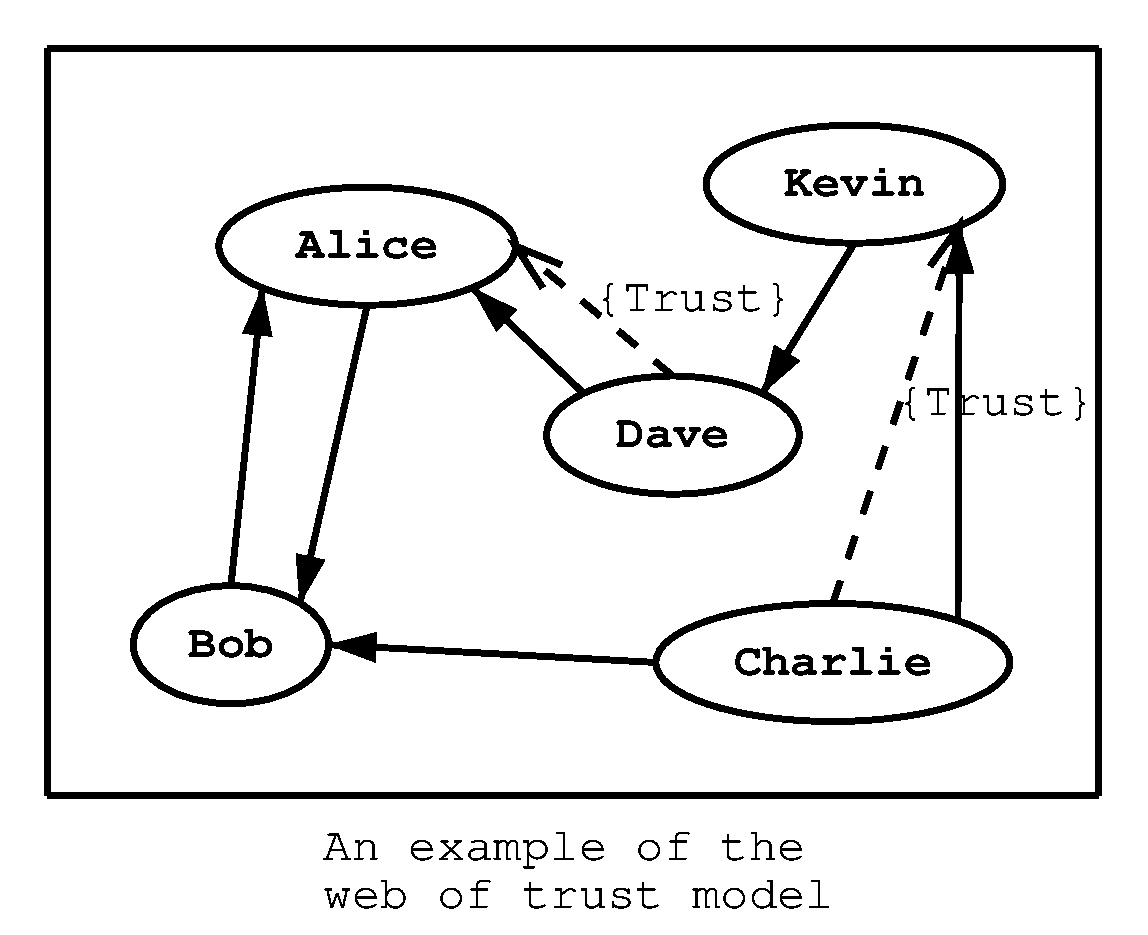
\includegraphics[height=9cm,width=11cm]{pgp-fig1}
\label{fig:pgp1}
\end{figure}

For example: If David trusts Alice to be an introducer, and Alice signed
Bob's key, Dave also trusts Bob's key to be the real one.

There are some key points that are important in that model. In the example
Alice has to sign Bob's key, only if she is sure that the key belongs
to Bob. Otherwise she may also make Dave falsely believe that this
is Bob's key. Dave has also the responsibility to know who to trust.
This model is similar to real life relations.

Just see how Charlie behaves in the previous example. Although he has 
signed Bob's key - because he knows, somehow, that it belongs to Bob - 
he does not trust Bob to be an introducer. Charlie decided to trust only 
Kevin, for some reason. A reason could be that Bob is lazy enough, and 
signs other people's keys without being sure that they belong to the 
actual owner.


\subsubsection{GnuTLS functions}

First we've to differ between owerntrust and validity. Sometimes trust
and validity is used as a synonym but this is not correct.
\par
The ownertrust describes how trustworthy the signature of a special
key owner is. Even if we've three or more signatures to make a key valid,
it's possible that we don't trust the owner at all and thus we don't trust 
the signature he made. There are different ownertrust levels:
\begin{enumerate}
\item Don't know
\item I do NOT trust
\item I trust marginally
\item I trust fully
\item I trust ulitmately.
\end{enumerate}

For example we need three marginal trusted signature to make a key
valid or one full trusted signature. The ultimate trust is only used
when we are the owner of a key and we also have the secret key.
\par
In the case we don't trust the owner, those signatures are skipped
for the web of trust calculation.
\par
All checks in GnuTLS are done in \printfunc{gnutls_openpgp_verify_key}{gnutls\_openpgp\_verify\_key}. 
If a trustdb is available, this is the file which contains all information about the
key owner (ownertrust), additional checks are performed.
\\
First we get the trustdb entry to see if the key is not disabled because
those keys shouldn't be used at all. Another possible case is that we
don't trust the key, which means we don't need to perform further checks.
\par
If the ownertrust is at least marginal we continue to check all signatures
the key contains to get the validity of the key. It is likely that the
public keyring does not contain all needed keys to check all signatures.
When a signature could not be checked due to a missing key, the function 
tries the next signature. When NO public key is available, the function
checks at least the self signature which must be valid in any case because
it was created by the key itself.
\\
Validity means if the signatures on the key are valid and the key was not 
changed by somebody or corrupted during transport.






\section{Anonymous authentication\index{Anonymous authentication}}
The anonymous key exchange perform encryption but there is no indication of 
the identity of the peer. This kind of authentication is vulnerable to a
man in the middle attack, 
but this protocol can be used even if there is no prior communication and
trusted parties with the peer, or when full anonymity is required.
Unless really required, do not use anonymous authentication.
Available key exchange methods are shown in \hyperref{figure}{figure }{}{fig:anon}.

\begin{figure}[hbtp]
\begin{tabular}{|l|p{9cm}|}

\hline
ANON\_DH & This algorithm exchanges Diffie Hellman parameters. 
\\
\hline
\end{tabular}

\caption{Supported anonymous key exchange algorithms}
\label{fig:anon}

\end{figure}

\section{Authentication using SRP\index{SRP authentication}}

Authentication using the SRP\footnote{SRP stands for Secure Remote Password and 
is described in \cite{RFC2945}. The SRP key exchange is not a part of the \tlsI{} protocol}
protocol is actually password authentication. The two peers can be identified using a
single password, or there can be combinations where the client is 
authenticated using SRP and the server using a certificate.
\par
The advantage of SRP authentication, over other proposed secure password 
authentication schemas, is that SRP does not require the server to hold
the user's password. This kind of protection is similar to the one used traditionally
in the \emph{UNIX} ``passwd'' file, where the contents of this file did not cause
harm to the system security if they were revealed.
The SRP needs instead of the plain password something called a verifier, 
which is calculated using the user's password, and if stolen cannot
be used to impersonate the user. See \cite{TOMSRP} for a detailed description
of the SRP protocol, and for the Stanford SRP libraries.

\par
The implementation in \gnutls{} is based on paper \cite{TLSSRP}.
The available key exchange methods are shown in \hyperref{figure}{figure }{}{fig:srp}.

\begin{figure}[hbtp]
\begin{tabular}{|l|p{9cm}|}

\hline
SRP & Authentication using the SRP protocol. 
\\
\hline
SRP\_DSS & Client authentication using the SRP protocol. Server is 
authenticated using a certificate with DSA parameters.
\\
\hline
SRP\_RSA & Client authentication using the SRP protocol. Server is 
authenticated using a certificate with RSA parameters.
\\
\hline
\end{tabular}

\caption{Supported SRP key exchange algorithms}
\label{fig:srp}

\end{figure}

If clients supporting SRP know the username and password before the connection,
should initialize the client credentials and call the
function \printfunc{gnutls_srp_set_client_credentials}{gnutls\_srp\_set\_client\_credentials}.
Alternatively they could specify a callback function by using the
function \printfunc{gnutls_srp_set_client_credentials_function}{gnutls\_srp\_set\_client\_credentials\_function}.
This has the advantage that allows probing the server for SRP support.
In that case the callback function will be called twice per handshake.
The first time is before the ciphersuite is negotiated, and 
if the callback returns a negative error code, the callback will be 
called again if SRP has been negotiated. 
This uses a special TLS-SRP handshake idiom in order to avoid, in
interactive applications, to ask the user for SRP password and username 
if the server does not negotiate an SRP ciphersuite.
\par
In server side the default behaviour of \gnutls{} is to read the usernames 
and SRP verifiers from password files. These password files are the ones used
by the \emph{srp libraries} and can be specified using the
\printfunc{gnutls_srp_set_server_credentials_file}{gnutls\_srp\_set\_server\_credentials\_file}.
If a different password file format is to be used, then the 
function \printfunc{gnutls_srp_set_server_credentials_function}{gnutls\_srp\_set\_server\_credentials\_function},
should be called, in order to set an appropriate callback.
\par
Some helper functions such as
\begin{itemize}
\item \printfunc{gnutls_srp_verifier}{gnutls\_srp\_verifier}
\item \printfunc{gnutls_srp_base64_encode}{gnutls\_srp\_base64\_encode}
\item \printfunc{gnutls_srp_base64_decode}{gnutls\_srp\_base64\_decode}
\end{itemize}
are included in \gnutls{}, and may be used to generate, and maintain
SRP verifiers, and password files. 
A program to manipulate the required parameters 
for SRP authentication is also included. See section \ref{srpcrypt} on 
page \pageref{srpcrypt} for more information.


